\section{Metodologia CRISP-DM}

De forma a garantir a qualidade dos modelos produzidos ao longo deste estudo, a metodologia \textit{Cross Industry Standard Process for Data Mining}, ou CRISP-DM, foi empreendida no intuito de garantir inclusão de abordagens normalmente utilizadas pelos profissionais da área com vantagens imediatas na qualidade do projecto desenvolvido.

\begin{figure}[H]
    \centering
    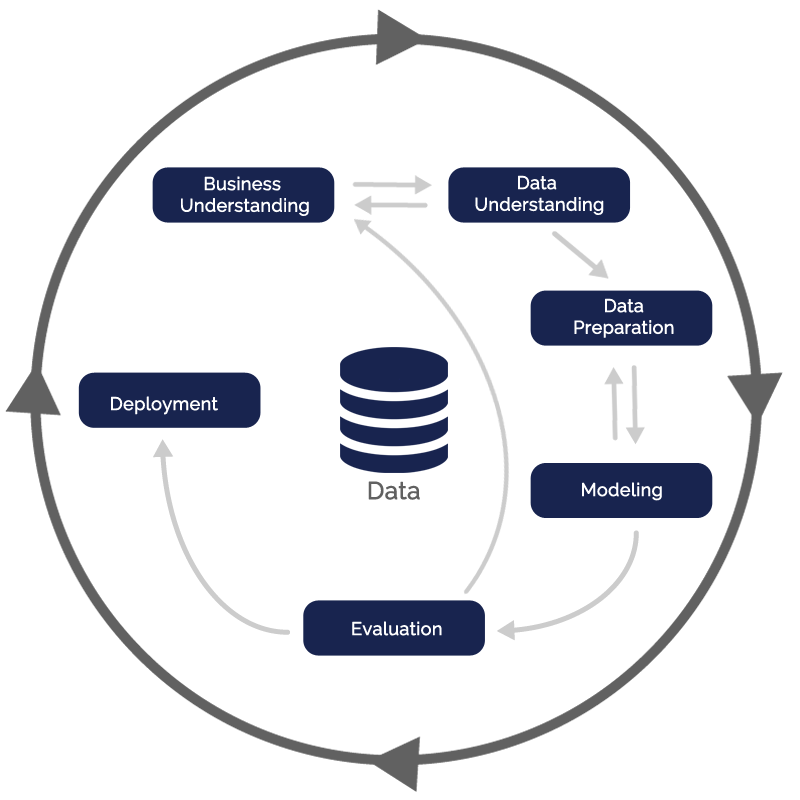
\includegraphics[width=0.4\linewidth]{Figures/crispdm.png}
    \caption{Diagrama ilustrativo da metodologia CRISP-DM.}
    \label{fig:s2i1}
\end{figure}

A figura \ref{fig:s2i1} ilustra os passos considerados por esta metodologia. De imediato, é possível perceber que esta metodologia não possui um início ou fim bem definido, propositadamente este comportamento é definido de forma a conseguir garantir que existe um refinamento do projecto ao longo do tempo, cada iteração contemplando das informações colectadas pela iteração anterior. Esta metodologia pode ser, resumidamente, descrita nos seguintes termos.

\begin{enumerate}
    \item \textbf{Compreensão do Negócio} - É importante perceber qual é o domínio do negócio/tema que estamos a considerar, o que estamos a tentar prever e como utilizar o nosso conhecimento de domínio em nosso prol.
    \item \textbf{Compreensão dos Dados} - Compreender o conjunto de dados captados, como os utilizar para alcançar o nosso objetivo e explorar estes de forma a descobrir fatores de interesse.
    \item \textbf{Preparação dos Dados} - Perceber qual a melhor forma para processar os dados de tal forma a que os modelos desenvolvidos possam tirar mais proveito.
    \item \textbf{Modelação} - Pesar os diferentes modelos utilizados, a diferenças entre si para alcançar o objetivo, bem como ponderar a variação dos hyper-parâmetros.
    \item \textbf{Apreciação} - Comparar o modelo com os objetivos iniciais propostos e perceber de que forma o modelo permite descrever o desejado.
\end{enumerate}

É importante ter em conta que a fase denotada como \textit{Deployment} da figura \ref{fig:s2i1} foi propositadamente deixada de parte, por não ter sido considerada em grande amplitude ao longo deste projeto.